\chapter{Sicurezza nelle reti}
Ci sono delle problematiche con cui chiunque può aver avuto a che fare come: danneggiamento dei computer connessi a internet mediante virus; violazioni di privacy; impossibilità di utilizzare servizi Internet.

\begin{redbar}
    Occuparsi di sicurezza vuol dire studiare come un malintenzionato può attaccare la rete o un host e adottare metodi di difesa o progettare nuove architetture che siano immuni da attacchi.
\end{redbar}

\section{Introduzione}
Un attacco spesso indicato anche come intrusione è un qualsiasi insieme di azioni che tenta di
compromettere l’integrità, la confidenzialità o la disponibilità di una risorsa. \textit{Ma quindi cosa vuol dire “comunicare in modo sicuro?”} Per comunicare in modo sicuro si vogliono mantenere le comunicazioni segrete, protette da ogni possibile intrusione. Fatte queste considerazioni, possiamo identificare le proprietà auspicabili per la comunicazione sicura.
\begin{itemize}
    \item \textit{Riservatezza o confidenzialità:} solo mittente e destinatario (che devono essere autenticati) devono essere in grado di comprendere il contenuto del messaggio che deve rimanere segreto;
    \item \textit{Integrità:} il contenuto della comunicazione non deve essere alterato;
    \item \textit{Disponibilità:} utenti legittimi devono poter usare i servizi di rete.
\end{itemize}

Programmi dolosi come virus, worm, ecc. possono introdursi all’interno di un host: tramite attachment in posta elettronica, scaricando programmi o applicazioni da Internet, sfruttando vulnerabilità di programmi già presenti sull’host... Generalmente per un buon risultato di un attacco si seguono dei passaggi:
\begin{itemize}
    \item \textit{Scansione della rete:} in questa fase si mira a recuperare più infomazioni possibili sulla rete obiettivo (Whois, dig, nslookup, Nmap - strumento di Network Mapping);
    \item \textit{Identificazione delle vulnerabilità:} scansione a livello di singoli host (servizi disponibili sui vari host, versione di sistema operativo, port scanning).
    \item \textit{Attacco:} vengono sfruttate vulnerabilità scoperte nella fase precedente, creando un punto di appoggio per un accesso futuro (creando un account, installando una backdoor);
    \item \textit{Espansione dell’attacco:} l’intruso accede nuovamente al sistema per rubare dati confidenziali, cancellando file, mettendo fuori uso il sistema (installazione di programmi dolosi, denial of service - DoS).
\end{itemize}

\subsection{Network mapping}
Il network mapping è un metodo per il recupero di informazioni sulla rete obiettivo, al fine di tracciare una mappa dei sistemi connessi e individuarne le vulnerabilità. Per essere effettivo deve aggirare le regole adottate dai firewall (e progredire con il loro aggiornamento). Storicamente è basato su ping e adotta meccanismi molto sottili per introdursi in una rete e ottenere un risultato analogo. L'obiettivo è ottenere in qualche modo una risposta dalle macchine sotto esame senza badare all’informazione ottenuta. I principali tipi di network mapping si suddividono in: metodi basati su richiesta valida e metodi basati su richiesta non valida.

I metodi basati su richiesta valida inviano una richiesta valida verso un servizio che comporta una risposta da parte del server che offre tale servizio (ad esempio una richiesta orario corrente). Si suddividono, a loro volta, in metodi che utilizzano:
\begin{itemize}
    \item \textit{TCP.} Sfruttano caratteristiche delle procedure di apertura e chiusura di una connessione (3-way handshake) con l'obiettivo di ricevere una qualche risposta (es. TCP ACK o TCP RST) che dimostri l’attività dell’host. Ad esempio: invio di TCP SYN verso una presunta porta aperta (ricevendo TCP SYN/ACK); invio di TCP flag che causano il ritorno di un TCP RST; invio di TCP ACK verso qualsiasi porta attiva; invio TCP FIN verso una porta che si suppone chiusa; invio di un TCP SYN/ACK (qualsiasi sia lo stato della porta); invio TCP XMAS su porta chiusa; invio TCP NULL su porta chiusa.
    \item \textit{UCP.} E' l'approccio meno utilizzato e meno affidabile. Ad esempio: UDP/Echo port: invio di UDP echo request; UDP Scan: invio pacchetto UDP verso porta chiusa causa risposta ICMP Port Unreacheable.
    \item \textit{ICMP.} ICMP è largamente usato per i mezzi che offre nel verificare se una destinazione è raggiungibile. Ad esempio: Icmp echo request (Ping); Icmp timestamp request; Icmp information request; Icmp Address Mask request.
\end{itemize}

I metodi basati su richiesta non valida prevedono l'invio di una richiesta non valida che viola la specifica dell’IP per ricevere un messaggio di errore dalla macchina. Può essere fatto inviando un primo frammento senza inviare i successivi e la macchina ricevente dopo un timeout risponde con un ICMP Fragment reassembly time exceeded, oppure specificando un valore non valido all’interno di uno qualsiasi dei campi dell’intestazione IP si ottiene un messaggio di errore ICMP dalla macchina destinataria.

Con il port scanning si ha una scansione dettagliata dei singoli host per scoprire i servizi attivi. Conosciuta la lista dei servizi attivi si possono individuare vulnerabilità sfruttabili per eventuali connessioni o attacchi. Si possono usare metodi simili a quelli nel network mapping (TCP SYN, TCP SYN/ACK, TCP FIN, ecc.).

\subsection{Attacchi}
I principali tipi di attacchi sono rivolti a: spiare la conversazione (\textit{sniffing}) per ottenere carte di credito, comunicazioni con la banca o informazioni di DNS e di routing; impersonare un altro soggetto (\textit{spoofing}); dirottare una sessione in corso (\textit{hijacking}); mettere fuori uso alcuni servizi (\textit{Denial of service}).

Il malware (malicious software) può raggiungere gli host attraverso virus, worm, o cavalli di Troia.
Un Malware di spionaggio può registrare quanto viene digitato, i siti visitati e informazioni di upload. Gli host infettati possono essere “arruolati” in botnet, e usati per lo spamming e per gli attacchi di DDoS. Il malware è spesso auto-replicante, da un host infettato può passare ad altri host.

I cavalli di Troia rappresentano la parte nascosta di un software utile. Oggi si trova spesso su alcune pagine web (ActiveX, plugin)... I virus sono infezioni che provengono da un oggetto ricevuto
(attachment di e-mail), e mandato in esecuzione, è auto-replicante ovvero si propaga da solo ad altri host e utenti. Un worm è un'infezione che proviene da un oggetto passivamente ricevuto
che si auto-esegue, anchè un worm è auto-replicante. Con al negazione di servizio (DoS) gli attaccanti fanno sì che le risorse (server, ampiezza di banda) non siano più disponibili al traffico legittimo sovraccaricandole di traffico artefatto. Questo viene fatto selezionando l’obiettivo, facendo irruzione negli host attraverso la rete e inviando pacchetti (flooding) verso un obiettivo da parte degli host compromessi.

Gli attaccanti che analizzano i pacchetti tramite packet sniffer sono passivi, infatti non immettono pacchetti sul canale, per cui sono difficili da individuare. Questa lettura dei pacchetti è più facile su mezzi broadcast (Ethernet condivisa, wireless) dove un’interfaccia di rete registra tutti i pacchetti (password comprese) che l’attraversano.

Gli attaccanti usano indirizzi sorgente falsi tramite l'IP spoofing: invio di pacchetti con un indirizzo sorgente falso.

Gli attaccanti registrano e riproducono con record-and-playback: “sniffano” dati sensibili
(password, ad esempio), per poi utilizzarli in un secondo tempo.

\section{Sicurezza operativa}
Le contromisure per tutti questi attacchi sono: antivirus, firewall e Intrusion detection system e
crittografia.

\subsection{Antivirus}
Un antivirus è un software atto a rilevare ed eliminare programmi dolosi (virus, worm, etc.). Viene installato sui singoli host per cui agisce localmente all’host, anche se ne esistono di altri tipi come antivirus per server (mail server).

Un antivirus esamina i dati interni al computer per rilevare presenza di programmi dolosi noti. Analizza il comportamento dei vari programmi alla ricerca di istruzioni sospette perché tipiche del comportamento dei virus. Deve essere sempre aggiornato con la creazione di nuovi attacchi (sempre un passo indietro agli attacchi). 

\subsection{Firewall}
\textit{E’ possibile prevenire i virus ovvero impedire che entrino nel sistema?} 

Un firewall è una struttura hardware e software che separa una rete privata dal resto di Internet e consente all’amministratore di controllare e gestire il flusso di traffico tra il mondo esterno e le risorse interne.

\begin{figure}[ht]
    \centering
    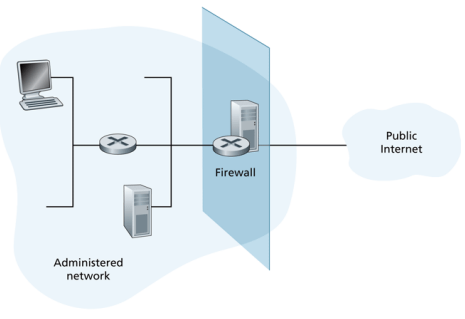
\includegraphics[width=8cm]{images/firewall.PNG}
    \caption{Rete amministrata e Internet separate da un firewall}
    \label{fig:firewall}
\end{figure}

Tutto il traffico verso l’interno e viceversa passa attraverso il firewall e solo al traffico
autorizzato sarà consentito passare.

Un firewall permette di: consentire solo accessi autorizzati all’interno della rete (una serie di utenti/host autenticati); prevenire attacchi di negazione del servizio, come SYN flooding, l’intruso stabilisce molte connessioni TCP fasulle per non lasciare risorse alle connessioni “vere”; prevenire modifiche/accessi illegali ai dati interni, ad esempio, l’intruso può sostituire l’homepage del MIUR con qualcos’altro.

Esistono tre tipi di firewall:
\begin{enumerate}
    \item \textit{A filtraggio dei pacchetti.} Una rete privata è collegata a Internet mediante un router. Il router è responsabile del filtraggio dei pacchetti e determina quali pacchetti devono essere bloccati o quali possono passare in base a: l'indirizzo IP sorgente o destinazione; le porte sorgente e destinazione TCP o UDP; il tipo di messaggio ICMP; i bit TCP SYN o ACK. 

    \begin{center}
    \begin{tabular}{|p{6cm}|p{7cm}|}
    \hline
    \textbf{Politica} & \textbf{Configurazione del firewall}\\\hline
    Nessun accesso web all’esterno & Bloccare tutti i pacchetti uscenti con qualsiasi indirizzo IP di destinazione e porta di destinazione 80\\\hline
    Nessuna connessione TCP entrante, eccetto quelle dirette al solo server web pubblico & Bloccare tutti i pacchetti TCP SYN entranti verso qualsiasi indirizzo IP tranne quelli verso l’indirizzo IP 130.207.244.203 e con porta destinazione 80\\\hline
    Evitare che le radio web consumino tutta la banda disponibile & Bloccare tutti i pacchetti UDP entranti, eccetto i pacchetti DNS\\\hline
    Evitare che la rete possa essere usata per un attacco DoS & Bloccare tutti i pacchetti ICMP ping diretti a un indirizzo broadcast (per esempio 130.207.255.255)\\\hline
    Evitare che la rete possa essere rilevata tramite Traceroute & Bloccare tutti i messaggi ICMP uscenti per TTL scaduto\\\hline
    \end{tabular}
    \end{center}

    ACL è una tabella di regole da applicare integralmente ai pacchetti entranti. Un esempio di ACL per organizzazione \texttt{222.22/16}:
    \begin{center}
    \begin{tabular}{|c|p{2cm}|p{2.05cm}|c|p{1.5cm}|p{1.5cm}|c|}
    \hline
    \textbf{Azione} & \textbf{Indirizzo sorgente} & \textbf{Indirizzo destinazione} & \textbf{Protocollo} & \textbf{Porta sorgente} & \textbf{Porta destinazione} & \textbf{Bit di flag}\\\hline
    consenti & \texttt{222.22/16} & al di fuori di \texttt{222.22/16} & TCP & $>$1023 & 80 & qualsiasi\\\hline
    consenti & al di fuori di \texttt{222.22/16} & \texttt{222.22/16} & TCP & 80 & $>$1023 & ACK\\\hline
    consenti & \texttt{222.22/16} & al di fuori di \texttt{222.22/16} & UDP & $>$1023 & 53 & -\\\hline
    consenti & al di fuori di \texttt{222.22/16} & \texttt{222.22/16} & UDP & 53 & $>$1023 & -\\\hline
    blocca & qualunque & qualunque & tutti & qualunque & qualunque & tutti\\\hline
    \end{tabular}
    \end{center}

    \item \textit{A filtraggio dei pacchetti con memoria dello stato.} Il filtraggio tradizionale è uno strumento poco flessibile. Il filtraggio con memoria dello stato, invece, tiene traccia dello stato di tutte le connessioni TCP. Traccia l’impostazione della connessione (SYN) e la terminazione (FIN): può così determinare se i pacchetti in entrata o in uscita “hanno senso” ovvero sono scambiati all’interno di connessioni esistenti. Nella tabella delle connessioni attive viene aggiunta una nuova colonna di verifica della connessione.

    \begin{center}
    \begin{tabular}{|p{1.1cm}|p{1.5cm}|p{2.05cm}|p{1.5cm}|p{1.5cm}|p{1.5cm}|p{1.2cm}|p{1.5cm}|}
    \hline
    \textbf{Azione} & \textbf{Indirizzo sorgente} & \textbf{Indirizzo destinazione} & \textbf{Protocollo} & \textbf{Porta sorgente} & \textbf{Porta destinazione} & \textbf{Bit di flag} & \textbf{Verifica della connessione}\\\hline
    consenti & \texttt{222.22/16} & al di fuori di \texttt{222.22/16} & TCP & $>$1023 & 80 & qualsiasi&\\\hline
    consenti & al di fuori di \texttt{222.22/16} & \texttt{222.22/16} & TCP & 80 & $>$1023 & ACK&X\\\hline
    consenti & \texttt{222.22/16} & al di fuori di \texttt{222.22/16} & UDP & $>$1023 & 53 & -&\\\hline
    consenti & al di fuori di \texttt{222.22/16} & \texttt{222.22/16} & UDP & 53 & $>$1023 & -&X\\\hline
    blocca & qualunque & qualunque & tutti & qualunque & qualunque & tutti&\\\hline
    \end{tabular}
    \end{center}
    
    \item \textit{A livello di applicazione (gateway).} Il filtraggio dei pacchetti consente di effettuare un controllo sulle intestazioni IP e TCP/UDP. Ad esempio permette ai client interni (autorizzati) le connessioni Telnet ma impedisce il contrario. Il gateway consente un filtraggio a livello di applicazione. Tutte le connessioni Telnet verso l’esterno devono passare attraverso il gateway. Il gateway non solo concede l’autorizzazione all’utente ma smista anche le informazioni fra l’utente e l’host. La configurazione del filtro del router blocca tutti i collegamenti eccetto quelli che riportano l’indirizzo IP del gateway.
\end{enumerate}

\begin{figure}[ht]
    \centering
    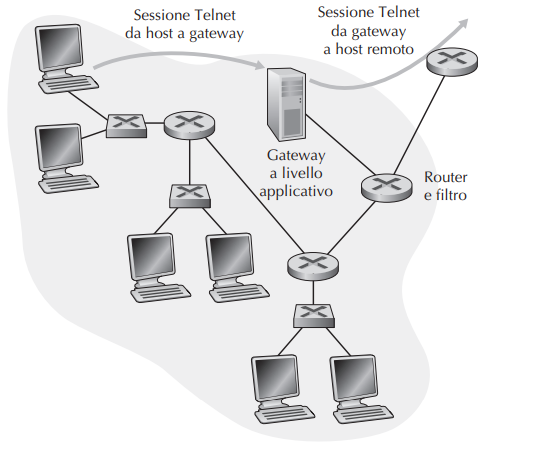
\includegraphics[width=8cm]{images/gateway.PNG}
    \caption{Firewall costituito da un gateway applicativo e da un filtro}
    \label{fig:gateway}
\end{figure}

\subsection{Intrusion detection system}
Un intrusion detection system (IDS)  è un sistema passivo che si basa sull’analisi del traffico di rete (non immette pacchetti in rete). Rileva un’ampia gamma di attacchi: guarda il contenuto dei pacchetti e li relaziona tra loro ed dsamina le correlazioni tra più pacchetti (scansione delle porte, scansione della pila TCP, attacchi DoS). Un IDS genera allarmi (ma non blocca il traffico) e si basa su un packet sniffer con l'aggiunta di un insieme di regole.

Una variante dell'intrusion detection system è il network based intrusion detection. Network-based è il sistema cattura e analizza il traffico di rete (SNORT). Ci sono anche sistemi host-based dove la sorgente di informazione è locale e interna a un host, in generale a livello di sistema operativo (file di log).

Il signature based IDS mantiene un database di firme degli attacchi (ovvero insieme di regole riguardanti un pacchetto o un insieme di pacchetti) e confronta ciascun pacchetto con le firme nel database. Se un pacchetto o una serie di pacchetti corrisponde a una firma nel database allora viene generato un allarme. Così facendo, però, si trova sempre un passo indietro rispetto a nuovi attacchi.

L'anomaly based IDS crea un profilo di traffico “normale” e genera un allarme quando rileva un comportamento (di rete) anomalo. Può rilevare nuovi attacchi ma non può avere elevati falsi positivi e falsi negativi.

L’IDS può essere composto da molteplici sistemi di rilevamento delle intrusioni e differenti tipi di
controllo in punti diversi.

\begin{figure}[ht]
    \centering
    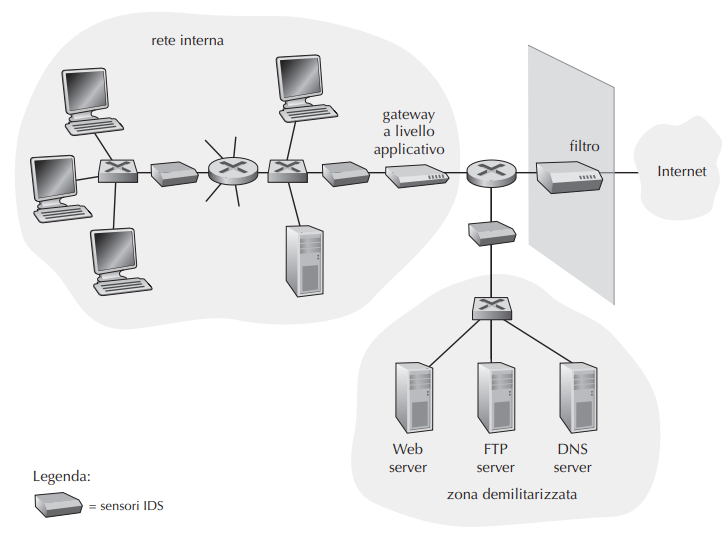
\includegraphics[width=10cm]{images/ids.PNG}
    \caption{Organizzazione che usa un filtro, un gateway applicativo e sensori IDS}
    \label{fig:ids}
\end{figure}

\section{Sicurezza nella comunicazione}
Possiamo identificare le proprietà auspicabili per la sicurezza nella comunicazione:
\begin{itemize}
    \item \textit{Riservatezza o confidenzialità:} solo mittente e destinatario devono comprendere il contenuto del messaggio;
    \item \textit{Autenticazione:} mittente e destinatario devono essere sicuri della loro identità;
    \item \textit{Integrità del messaggio:} mittente e destinatario devono essere sicuri che il contenuto non subisca alterazioni durante la trasmissione (per cause fortuite o per manipolazioni);
    \item \textit{Disponibilità e controllo dell’accesso:} un servizio deve essere accessibile a chi è legittimamente autorizzato.
\end{itemize}

Uno scenario ben noto nel mondo della sicurezza di rete vede Roberto e Alice che vogliono comunicare in modo sicuro e un intruso può intercettare, rimuovere, aggiungere messaggi o modificare
il loro contenuto. Nella vita reale Alice e Roberto possono essere: un browser/server Web durante una transazione elettronica (es. un acquisto on-line); un client/server di banche on-line; un server DNS; dei sistemi che si scambiano tabelle d’instradamento.

\begin{figure}[ht]
    \centering
    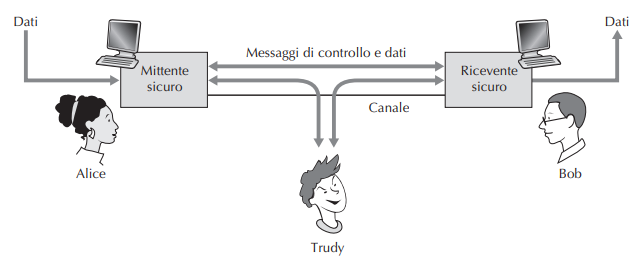
\includegraphics[width=11cm]{images/sicurezza-comunicazione.PNG}
    \caption{Mittente, ricevente e intruso}
    \label{fig:sicurezza-comunicazione}
\end{figure}

A questo punto un malintenzionato potrebbe, come abbiamo già visto, procedere con una delle seguenti azioni: spiare: intercettare i messaggi, aggiungere messaggi e sovraccaricare il sistema, impersonare un altro soggetto, dirottare una sessione in corso e sostituirsi al mittente o al destinatario, negare il servizio.

\subsection{Principi di crittografia}
La crittografia permette di trasformazione dei messaggi per renderli sicuri e immuni agli attacchi garantendo confidenzialità e riservatezza.

\begin{figure}[ht]
    \centering
    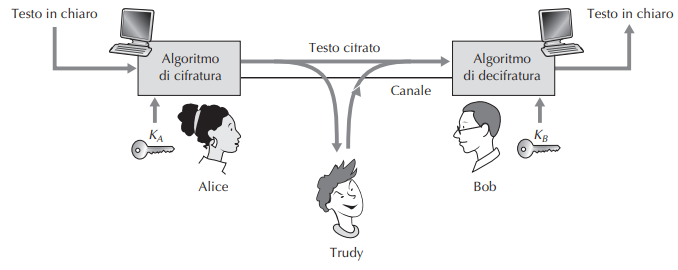
\includegraphics[width=11cm]{images/crittografia.PNG}
    \caption{Componenti crittografici}
    \label{fig:crittografia}
\end{figure}

Nei cosiddetti sistemi a chiave simmetrica la chiave per la cifratura e decifratura è la stessa e
può essere usata per comunicazione bidirezionale (da cui il termine simmetrica). Nei sistemi a chiave asimmetrica si usa una coppia di chiavi associate al destinatario: la chiave di cifratura è pubblica e la chiave di decifratura è privata. Si stabilisce una comunicazione unidirezionale con una coppia di chiavi.

\begin{figure}[ht]
    \centering
    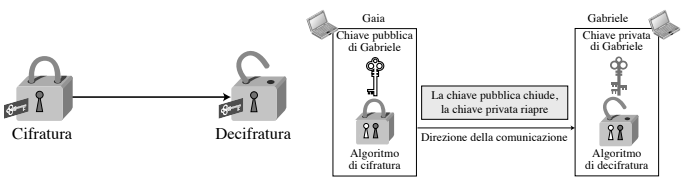
\includegraphics[width=11cm]{images/chiave-simmetrica-asimmetrica.PNG}
    \caption{Cifratura a chiave simmetrica e asimmetrica}
    \label{fig:chiave-simmetrica-asimmetrica}
\end{figure}

\subsection{Crittografia a chiave simmetrica}
Per cifrare il messaggio è necessario un algoritmo di cifratura e una chiave simmetrica condivisa. Per decifrare il messaggio è necessario un algoritmo di decifratura e una chiave simmetrica condivisa. La chiave simmetrica condivisa è segreta e deve essere scambiata a priori.

\begin{figure}[ht]
    \centering
    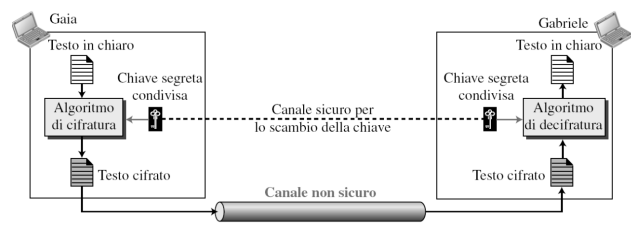
\includegraphics[width=11cm]{images/chiave-simmetrica.PNG}
    \caption{Cifratura a chiave simmetrica}
    \label{fig:chiave-simmetrica}
\end{figure}

\subsubsection{Algoritmi crittografici a sostituzione}
Un algoritmo crittografico a sostituzione sostituisce un simbolo con un altro.

Il cifrario monoalfabetico più semplice è quello a scorrimento (o additivo). Si ipotizzi che il testo in chiaro consista di lettere minuscole (dalla a alla z) e che il testo cifrato consista di lettere maiuscole (dalla A alla Z). Per poter effettuare delle operazioni matematiche sui testi in chiaro e cifrato si assegna un valore numerico a ciascuna lettera (minuscola e maiuscola).

\begin{figure}[ht]
    \centering
    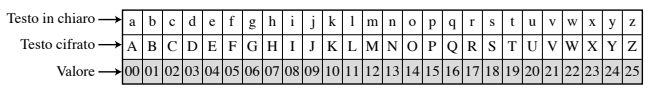
\includegraphics[width=11cm]{images/cifrario-scorrimento.PNG}
    \caption{Rappresentazione dei caratteri cifrato in modulo 26}
    \label{fig:cifrario-scorrimento}
\end{figure}

A ogni carattere (minuscolo o maiuscolo) viene assegnato come codice corrispondente un intero modulo 26. Anche la chiave segreta condivisa è un intero modulo 26. L'algoritmo crittografico aggiunge la chiave al codice del carattere del testo in chiaro, l'algoritmo di decifratura sottrae la chiave dal codice del carattere del testo cifrato. Tutte le operazioni vengono eseguite modulo 26.

\begin{Example}{Cifratura simmetrica}{}
    \textit{Crittografare il messaggio "hello" utilizzando il cifrario a scorrimento con chiave 15.}

    Si applica l'algoritmo al testo in chiaro, carattere per carattere:
    
    \begin{minipage}{\textwidth}
        \centering
        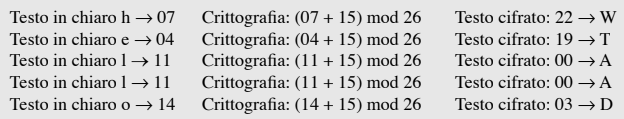
\includegraphics[width=0.8\textwidth]{images/es-cifratura-simmetrica.PNG}
        %\captionof{figure}{Esempio}
    \end{minipage}

    Il risultato è "WTAAD". Si noti che il cifrario è monoalfabetico poiché le due istanze del medesimo carattere del testo in chiaro "I" vengono crittografate in uno stesso carattere ("A") del testo cifrato. Per decifrare si utilizza lo stesso cifrario e la chiave 15.
    
    \begin{minipage}{\textwidth}
        \centering
        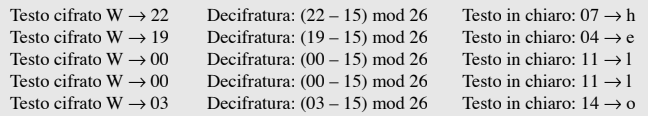
\includegraphics[width=0.8\textwidth]{images/es-cifratura-simmetrica2.PNG}
        %\captionof{figure}{Esempio}
    \end{minipage}
\end{Example}

I cifrari a scorrimento sono vulnerabili agli attacchi a forza bruta, che ricercano esaustivamente tutte le possibili chiavi. Lo spazio delle chiavi del cifrario a scorrimento è estremamente limitato: vi sono in totale 26 chiavi, ma la chiave 0 è inutile (il testo cifrato risulta uguale al testo in chiaro). Vi sono dunque solo 25 possibili chiavi. Sarebbe banale per un intruso sferrare un attacco a forza bruta sul testo cifrato.

Una soluzione migliore consiste nel creare un cifrario monoalfabetico a sostituzione dove si sostituisce una lettera con un'altra senza seguire un ordine di incremento.

\begin{Example}{Cifratura a sostituzione}{}
    \begin{minipage}{\textwidth}
        \centering
        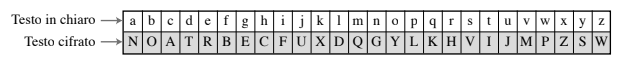
\includegraphics[width=0.8\textwidth]{images/es-cifratura-sostituizione.PNG}
        %\captionof{figure}{Esempio}
    \end{minipage}

    E' possibile utilizzare la chiave della figure per cifrare il messaggio:

    \begin{minipage}{\textwidth}
        \centering
        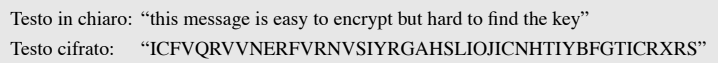
\includegraphics[width=0.8\textwidth]{images/es-cifratura-sostituizione2.PNG}
        %\captionof{figure}{Esempio}
    \end{minipage}
    
    E’ comunque vulnerabile: sebbene le chiavi siano molte di più ($26!$) è comunque possible un attacco a forza bruta che determina la frequenza relativa delle lettere e la confronta con la distribuzione standard della frequenza per la lingua in questione.
\end{Example}

\subsubsection{Cifrari a trasposizione}
Un cifrario a trasposizione non sostituisce un simbolo con un altro, ma ne cambia la posizione. Un simbolo nella prima posizione del testo in chiaro potrebbe figurare nella decima posizione del testo cifrato, un simbolo nell'ottava posizione del testo in chiaro potrebbe figurare nella prima posizione del testo cifrato. In altre parole un cifrario a trasposizione riordina, o traspone, i simboli.

\begin{figure}[ht]
    \centering
    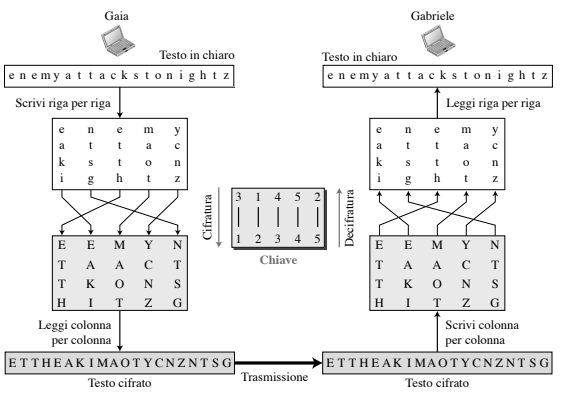
\includegraphics[width=11cm]{images/cifrario-trasposizione.PNG}
    \caption{Cifrario a trasposizione}
    \label{fig:cifrario-trasposizone}
\end{figure}

\subsubsection{Cifrario a blocchi}
Cifrario a blocchi. Un cifrario a blocchi cifra un intero gruppo di simboli del testo in chiaro per ottenere un gruppo di testo cifrato della medesima dimensione. Secondo questa definizione un cifrario a blocchi utilizza un'unica chiave per crittografare l'intero blocco, anche se la chiave è costituita da più valori. In un cifrario di questo tipo un blocco di testo cifrato dipende dall'intero blocco di testo in chiaro.

\begin{figure}[ht]
    \centering
    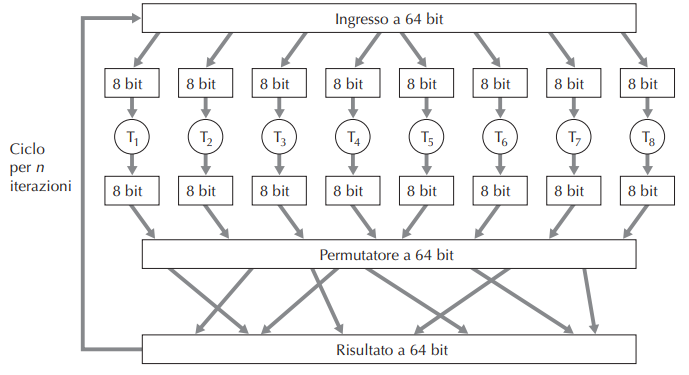
\includegraphics[width=11cm]{images/cifrario-blocchi.PNG}
    \caption{Cifrario a blocchi}
    \label{fig:cifrario-blocchi}
\end{figure}

\subsection{Crittografia a chiave asimmetrica (o pubblica)}
La crittografia a chiave simmetrica richiede che mittente e destinatario condividano una chiave segreta. Come si concorda la chiave (specialmente se i due interlocutori non si sono mai “incontrati”)? L’algoritmo di cifratura a chiave simmetrica lavora su numeri e su due chiavi diverse.

\begin{figure}[ht]
    \centering
    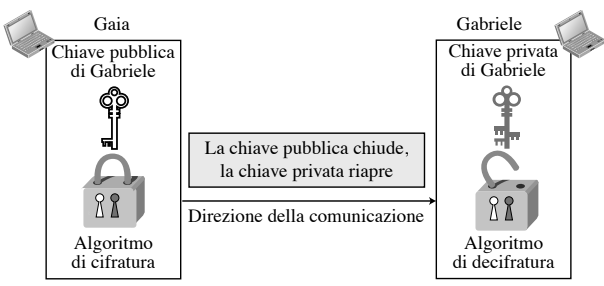
\includegraphics[width=9cm]{images/chiave-asimmetrica.PNG}
    \caption{Cifratura a chiave asimmetrica}
    \label{fig:chiave-asmmiterica}
\end{figure}

\begin{figure}[ht]
    \centering
    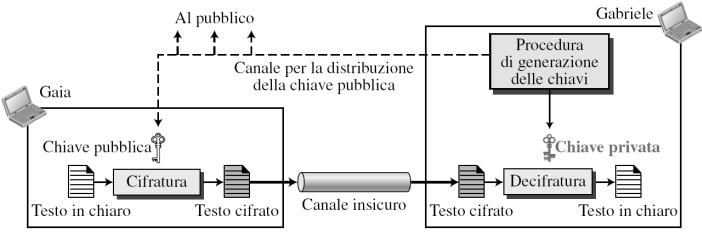
\includegraphics[width=9cm]{images/idea-geniale.PNG}
    \caption{L'idea geniale della crittografia asimmetrica}
    \label{fig:idea-geniale}
\end{figure}

La Figura \ref{fig:idea-geniale} schematizza l'idea generale della crittografia asimmetrica nel caso della cifratura. La figura evidenzia alcuni fatti importanti. In primo luogo pone in risalto la natura asimmetrica del cifrario. La responsabilità di garantire la sicurezza ricade principalmente sul destinatario (Gabriele in questo caso) che deve creare due chiavi una privata e una pubblica Gabriele ha il compito di distribuire la propria chiave pubblica alla comunità, per esempio tramite un canale di distribuzione della chiave pubblica.

In secondo luogo la crittografia asimmetrica implica che Gabriele e Gaia non possano utilizzare la stessa coppia di chiavi per la comunicazione bidirezionale: ciascun membro della comunità deve creare la propria coppia di chiavi pubblica e privata. 

Infine, la crittografia asimmetrica comporta che Gabriele abbia bisogno di una sola chiave privata per poter ricevere comunicazioni da qualsiasi membro della comunità, mentre Gaia deve utilizzare $n$ chiavi pubbliche per poter comunicare con $n$ membri della comunità, una per ciascuno di essi.

La crittografia asimmetrica è solitamente impiegata per cifrare/decifare quantità limitate di informazioni (es. la chiave di un cifrario simmetrico). Il testo in chiaro e il testo cifrato sono considerati numeri interi, la cifratura e la decifratura sono funzioni matematiche, il testo cifrato può essere inteso come $C = f(K_{pubb}, P)$, il testo in chiaro può essere inteso come $P = g(K_{priv}, C)$. RSA (Rivest, Shamir, Adleman) è un algoritmo a chiave asimmetrica largamente
diffuso.

\subsubsection{RSA}
Per la scelta delle chiavi si seguono questi passi:
\begin{enumerate}
    \item Scegliere due numeri primi di valore elevato: $p$, $q$ (es.: 1024 bit ciascuno).
    \item Calcolare $n = pq$, $z = (p-1)(q-1)$.
    \item Scegliere $e$ (con $e < n$) tale che non abbia fattori in comune con $z$ ($e$, $z$ sono “relativamente primi”).
    \item Scegliere $d$ tale che $ed-1$ sia esattamente divisibile per $z$ (in altre parole: $ed\mod z = 1$).
    \item La chiave pubblica è $(n,e)$, quella privata è $(n,d)$.
\end{enumerate}

\begin{figure}[ht]
    \centering
    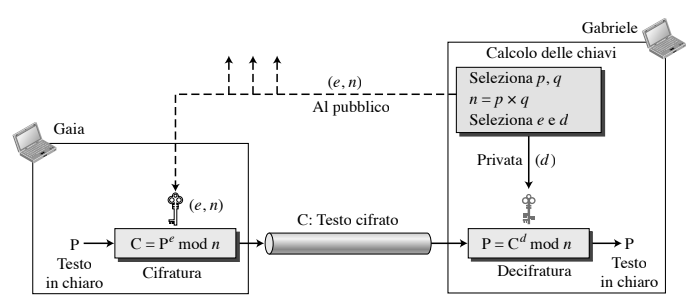
\includegraphics[width=9cm]{images/schema-rsa.PNG}
    \caption{Schema RSA}
    \label{fig:schema-rsa}
\end{figure}

Dati $(n,e)$ e $(n,d)$ calcolati come abbiamo appena visto, per la codifica di $m$ si calcola $c = m^e\mod n$, per decifrare il messaggio ricevuto, $c$, si calcola $m = c^d\mod n$.

\begin{equation*}
    m=(m^e\mod n)^d\mod n
\end{equation*}

\begin{Example}{RSA}{}
    \textit{Si supponga che Gabriele scelga $p=7$ e $q=11$, $n=35$ e $z=24$.}

    Si prenderanno $e=5$ così $e$ e $z$ sono relativamente primi, e $d=29$ così $ed-1$ è esattamente divisibile per $z$.
    \begin{center}Cifratura: 
    \begin{tabular}{c c c c c}
         lettera&$m$&$m^e$&$c=m^e\mod n$\\
         I&12&1524832&17
    \end{tabular}
    \end{center}
    \begin{center}Decifratura: 
    \begin{tabular}{c c c c c}
         $c$&$c^d$&$m=c^d\mod n$&lettera\\
         17&481968572106750915091411825223071697&12&I
    \end{tabular}
    \end{center}
\end{Example}

Osserviamo la seguente formula:
\begin{equation*}
    K_{priv}(K_{pubb}(m)) = m = K_{pubb}(K_{priv}(m))    
\end{equation*}

Notiamo che se si usa prima la chiave pubblica, e poi quella privata o se si usa prima la chiave privata, e poi quella pubblica il risultato non cambia.

\subsection{Integrità del messaggio}
Gabriele riceve un messaggio da Gaia, e vuole essere sicuro che: il messaggio  provenga effettivamente da Gaia; il messaggio non sia stato alterato lungo il cammino. Si possono usare funzioni hash crittografiche che prende in input $m$, produce un valore a lunghezza fissa, $H(m)$. Deve essere computazionalmente impossibile trovare due messaggi $x$ e $y$ tali che $H(x) = H(y)$ o anche dato $m = H(x)$, (con $x$ sconosciuta), è impossibile determinare $x$.

Garantisce integrità (il messaggio non è stato cambiato). Funzione hash che produce digest (immagine compressa del messaggio). Viene inviato sia il messaggio, sia il digest il messaggio viaggia in chiaro.

\begin{figure}[ht]
    \centering
    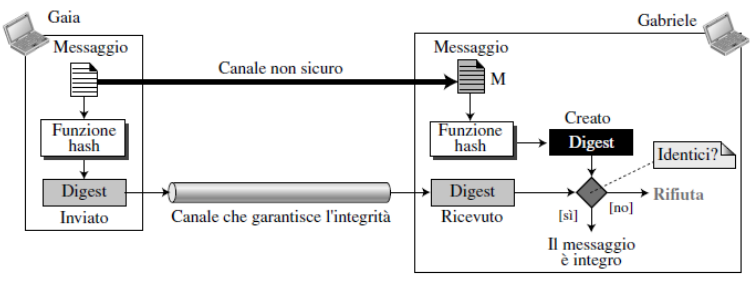
\includegraphics[width=9cm]{images/message-digest.PNG}
    \caption{Messaggio e relativo digest}
    \label{fig:message-digest}
\end{figure}

MD5 è molto usato per l’hash dei messaggi (RFC 1321), MD sta per Message Digest. Calcola una hash di 128 bit con un processo a 4 fasi. Con una stringa $x$ di 128 bit arbitrari, appare difficile costruire un messaggio $m$ il cui hash MD5 sia uguale a $x$. È molto usato anche Secure Hash Algorithm (SHA), Standard statunitense. Produce una sintesi del messaggio di 160 bit.

\subsection{Autenticazione ent-to-end}
Per autenticare l’origine del messaggio (il messaggio è stato scritto da Gaia)  viene inserito un codice segreto condiviso tra Gaia e Gabriele. Messaggio con chiave segreta vengono compressi con una hash crittografica per creare un Message Authentication code (MAC).

\begin{figure}[ht]
    \centering
    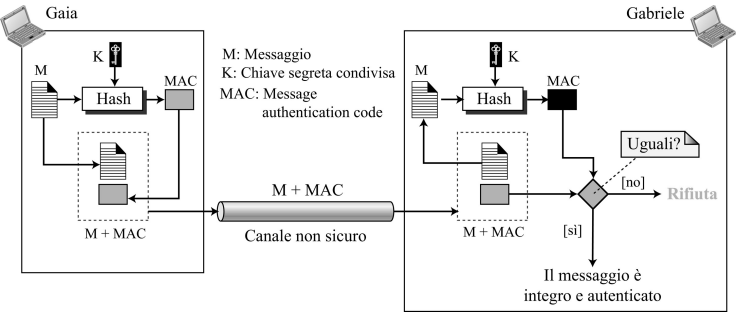
\includegraphics[width=9cm]{images/autenticazione-mac.PNG}
    \caption{Codice di autenticazione di messaggio (MAC)}
    \label{fig:autenticazione-mac}
\end{figure}

Un intruso può vedere il messaggio ma non può formularne uno nuovo per sostituire il precedente perchè non possiede la chiave segreta.

\subsubsection{Firma digitale}
Tecnica crittografica analoga all’invio di una tradizionale “firma scritta”. Altro modo di garantire integrità e autenticazione di un messaggio. Il mittente firma digitalmente un documento, stabilendo che lui è l’unico proprietario/creatore del messaggio. Verificabile e non falsificabile: il destinatario può dimostrare che il mittente e nessun altro può aver firmato il documento. Avviene mediante l’uso di una coppia di chiave pubblica e privata di chi firma.

Gaia firma un messaggio $M$, cifrandolo con la sua chiave privata, creando così un messaggio “firmato”, Gabriele decifra il messaggio applicando la chiave pubblica di Gaia. E' il meccanismo di crittografia asimmetrica applicata in modo inverso.

\begin{figure}[ht]
    \centering
    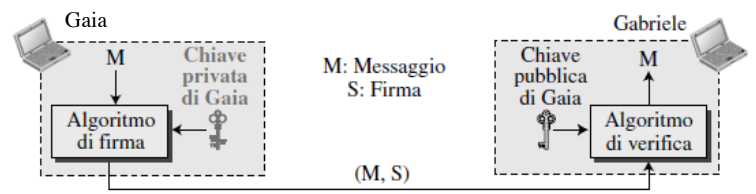
\includegraphics[width=9cm]{images/firma-digitale.PNG}
    \caption{Processo della firma digitale}
    \label{fig:firma-digitale}
\end{figure}

E' impossibile firmare un messaggio di un’altra persona a meno che non si conosca la sua chiave segreta. La firma digitale garantisce la proprietà di non ripudio: Gaia non può negare di aver firmato il documento e Gabriele può verificare che: Gaia ha firmato M; nessun altro ha firmato M; Gaia ha firmato M e non M’. Poiché la crittografia asimmetrica è inefficiente su messaggi lunghi, in genere si applica la firma digitale a un MESSAGE DIGEST.

\begin{figure}[ht]
    \centering
    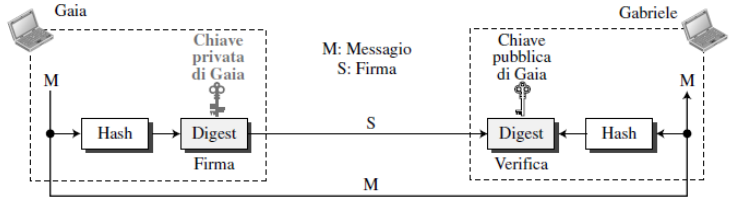
\includegraphics[width=9cm]{images/firma-digest.PNG}
    \caption{Firma del digest}
    \label{fig:firma-digest}
\end{figure}

Problema per la crittografia a chiave pubblica: quando Gaia riceve la chiave pubblica di Gabriele (attraverso una chiave USB, il sito web o via e-mail), come fa a sapere che è veramente la chiave pubblica di Gabriele e non quella di qualcun altro? Soluzione: autorità di certificazione (CA, certification authority).

Autorità di certificazione (CA): collega una chiave pubblica a una particolare entità. Gabriele registra la sua chiave pubblica con CA. Gabriele fornisce una “prova d’identità” a CA. CA crea un certificato che collega Gabriele alla sua chiave pubblica. Il certificato contiene la chiave pubblica di Gabriele con firma digitale di CA (CA dice “questa è la chiave pubblica di Gabriele”).